\documentclass[12pt]{article}
\usepackage[utf8]{inputenc}
\usepackage{lmodern}
\usepackage[french]{babel}
\usepackage{graphicx}
\usepackage{amsmath}
\usepackage{geometry}
\usepackage[export]{adjustbox}
\usepackage{xcolor}
\usepackage{float}
\usepackage{amssymb}

\title{Signal avancé}

\begin{document}

\maketitle

\section{Filtrage optimal / adaptatif}
\subsection{Problème de Wiener}
Norbert Wiener (1945) prédicition : traitement du signal statistique et réseaux de neurones artificiels.

\begin{figure}[H]
    \centering
    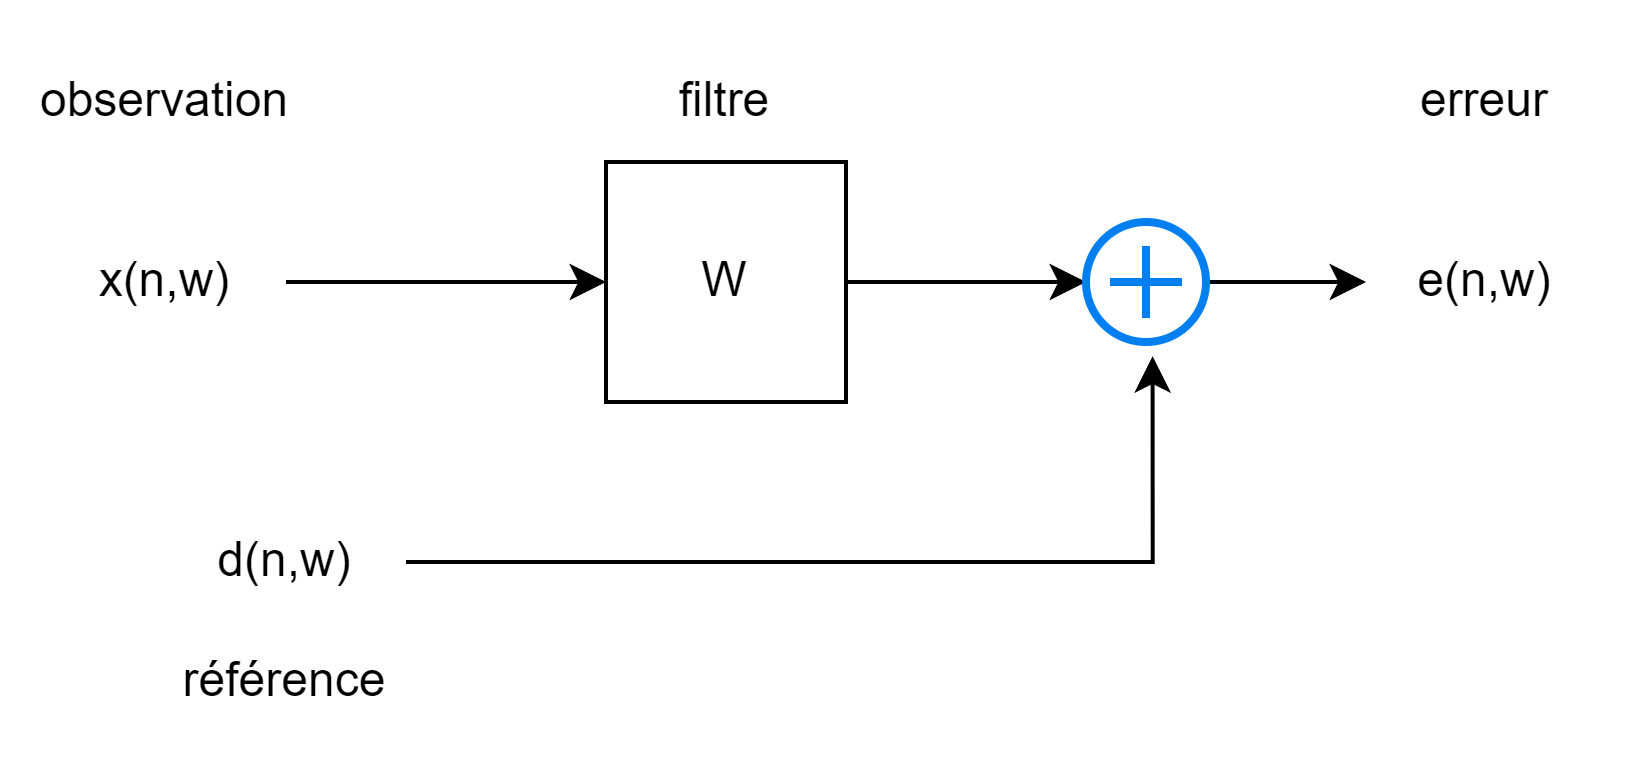
\includegraphics[width=0.8\linewidth]{image.png}
    \caption{Enter Caption}
    \label{fig:enter-label}
\end{figure}
Problème de Wiener : trouver $w$ pour minimiser l'erreur.
\begin{equation}
   \arg \min_{x} var(e(n,\omega)) \nonumber
\end{equation}
avec $var(e(n,\omega) \in \mathbb{R}$ 
$$var(e(n,\omega)) = E[\lvert e(n,\omega)-m_e(n)^2 \rvert]$$
avec $w_e(n) = E[e(n,\omega)]$\\
Rappel : la variance est la distance sur les processus. 
$$y(n,\omega) = w+ x(n,\omega) = \sum_k w_k x(n-k,w)$$ avec $w_k$ la réponse impulsionnelle.\\
Exemple : annulation d'écho accoustique en visiophonie.\\
$echoaccoustiques = \sum_{l=1}^L \alpha_l x(n-l,w)$
$$d(n,\omega) = b(n,\omega) + \sum_{l=1}^L \alpha_l x(n-l,w)$$

\begin{align}
        e(n,\omega) &= w + x(n,\omega) - d(n,\omega) \nonumber \\
        &= - b(n,\omega) + \sum_k (w_k - \alpha_k) x(n-k,w) \nonumber
\end{align}
Si $w_k = \alpha_k \Rightarrow e(n,\omega) = -b(n,\omega)$\\

\textbf{Objectif :} \\
- apprendre les bons $w_k$ à l'aide de $x(n,\omega)$ et $d(n,\omega)$ avec $n=0,1 ...N-1$ et de leurs statiques \\
- adapter aux variatbles dans le temmps\\
\textbf{Exemple 2 :} prédiction linéaire\\
$d(n,\omega) = x(n+1,w)$ à 1 pas\\
ou $d(n,\omega) = x(n+2, w)$ ou $x(n+h,w)$ à h pas.
\newpage

\subsection{Principe du filtre de Winener (statistiquement)}
\textbf{Hypothèses :} $x$ stationnaire au 2e ordre et $x$ et $d$ sont mutuellement stationnnaires. \\
\textbf{But :} Ici nous cherchons à minimiser w  $$E[\lvert e_c(n,\omega)\rvert ^2] = var(e_c(n,\omega)) = J(w)$$\\
$$e_c(n,\omega) = \sum_{k\in D} w_k x_c(n-k,w) - d_c(n,\omega)$$
\begin{figure}[H]
    \centering
    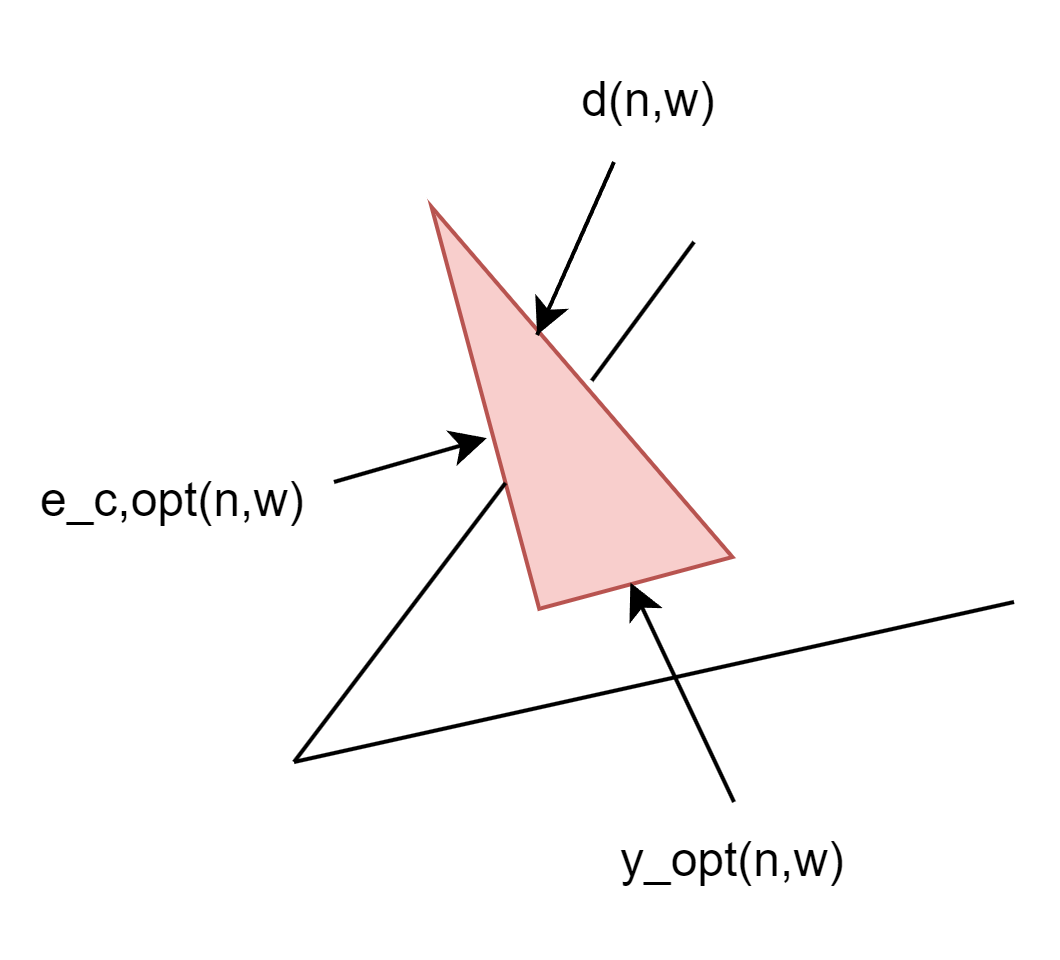
\includegraphics[width=0.5\linewidth]{image2.png}
\end{figure}
$y_{c,opt}(n,\omega) \in x_n$ et $x_n = $ espace des combinaisons linéaires des $x_c(n-k,w) \, k \in D \subset \mathbb{Z}$\\
$y_{c,opt}(n,\omega) = \sum_{k\in D} w_{opt,k} x_c(n-k,w)$ projection orthogonal de $d(n,\omega)$ sur $x_n$ (minimise la distance entre d et $x_n$).\\
Décorrélé $\forall k \in D$
\begin{equation}
    e_{c,opt}(n,\omega) \perp x_n \\
    \Leftrightarrow \Gamma_{opt,x}(n,n-k) = E[e_{c,opt}(n,\omega) \overline{x_c(n-k,w)}] =0   \nonumber
\end{equation}
équation de wiener-Hopf
$$\Leftrightarrow  E[(\sum_{l\in D} w_{opt,l} x_c(n-l, w) -d_c(n,\omega)) \overline{x_c(n-k,w)}]=0$$
$$\Leftrightarrow  \sum_{l\in D} w_{opt,l} E[x_c(n-l, w)\overline{x_c(n-k,w)}] = E[d_c(n,\omega)) \overline{x_c(n-k,w)}]$$
Par identification des fonctions de covariance  : 
$$\Leftrightarrow  \sum_{l\in D} w_{opt,l} \Gamma  = E[d_c(n,\omega)) \overline{x_c(n-k,w)}]$$

x est stationnaire du second ordre, on a donc : 
$$\Gamma_x(n-l,n-k) = \gamma_x(n-l-(n-k))=\gamma_x(k-l)$$
x et d sont mutuellement stationnaires :
$$\Gamma{d,x}(n,n-k) = \gamma_{d,x}(n-(n-k)) = \gamma_{d,x}(k)$$ fonction d'intercorrélation entre d et x
$$\Leftrightarrow \boxed{\sum_{l\in D} w_{opt,l} \gamma_x(k-l) = \gamma_{d,x}(k) \forall k \in D}$$
On en déduit plusieurs éléments :
\begin{itemize}
    \item l'equation est linéaire en $w_{opt}$ donc solvable
    \item nombre d'inconnues = card(D) = nombre d'équations.
    \item si det $\neq 0$ et 1 seule solution
\end{itemize}
\textbf{1er cas :} $D = \mathbb{Z}$\\
$$\sum_{l=-\infty}^{+\infty} w_{opt,l} \gamma_x(k-l)=\gamma_{d,x}(k) \forall \mathbb{Z}$$
$$\Leftrightarrow w_{opt}+\gamma_x(k) = \gamma_{d,x}(k) \forall k \in \mathbb{Z}$$
En passant à la TFTD : 
$$\mathring{w}_{opt}(\nu) \mathring{\gamma_x}(\nu)=\mathring{\gamma_{d,x}}(\nu)$$
ie $$\text{Réponse en fréquence x DSP } = \text{ Interspectre}$$
avec $$\mathring{\gamma_x}(\nu)= \sum_{k \in \mathbb{Z}} \gamma_x(k) e^{-j2\pi \nu k}$$\\
$\nu$ étant la fréquence réduite.
On en déduit alors la relation du filtre de Wiener doublement infini :
$$\boxed{\mathring{w}_{opt}(\nu) = \frac{\mathring{\gamma_{d,x}}(\nu)}{\mathring{\gamma_x}(\nu)}}$$ sur les fréquences où la DSP de $x$ est non nulle (sur les autres fréquence, ce n'est pas important puisque la DSP du signal filtré est nulle.\\
\textbf{Exercice :} Cas de l'annulation d'écho accoustique :
$$d(n,\omega) = b(n,\omega) + \sum_{l=1}^L \alpha_l x(n-l,w)$$
Calculer $\mathring{w_{opt}}(\nu)$. Sous quelles hypothèses, a-t-on $w_{opt} = \alpha$ ?
\\
On pose l'hypothèse que d et x sont mutuellement stationnaire. nous vérifirons cette hypothèse par la suite des calculs.\\
On a 
\begin{align}
    \Gamma_{d,x}(n,n-k) &= E\left[ (b_c(n,\omega)+ \sum_l \alpha_l (n-l,w)) \overline{x_c} (n-k,w) \right] \nonumber \\
    &= E[b_c \overline{x_c}] + \sum_l \alpha_l E\left[ x_c(n-l,w) \overline{x_c}(n-k,w) \right] \nonumber \\
    &= \Gamma_{b,x}(n,n-k) + \sum_l \alpha_l \Gamma_x(n-l,n-k) \nonumber 
\end{align}
En supposont b et x mutulement stationnaire, nous avons :
\begin{align}
    \Gamma_{d,x}(n,n-k) &= \gamma_{b,x}(k) + \sum_l \alpha_l \gamma_x(k-l) \text{ (Nous reconnaissons le produit de convolution)} \nonumber \\
    &= \gamma_{b,x}(k) + \alpha * \gamma_x(k) \text{ (ne dépend plus de n, hypothèse vérifiée)} \nonumber \\
    &= \gamma_{d,x}(k) \nonumber 
\end{align}
On applique la TF : \\
\begin{align}
    \mathring{\gamma}_{d,x}(\nu) \nonumber &= \mathring{\gamma}_{b,x}(\nu) + \mathring{\alpha} * \mathring{\gamma_x}(\nu) \nonumber 
\end{align}
\begin{align}
    \mathring{w}_{opt} (\nu) &= \frac{\mathring{\gamma_{b,x}}(\nu)}{\mathring{\gamma_x}(\nu)} + \mathring{\alpha}(\nu) \nonumber \\
    \text{Si } \frac{\mathring{\gamma_{b,x}}(\nu)}{\mathring{\gamma_x}(\nu)} = 0 \nonumber \\ &\Leftrightarrow \mathring{\gamma_{b,x}}(\nu) = 0 \nonumber \\
    &\Leftrightarrow \gamma_{b,x}(k) = 0  \nonumber \\
    &\Leftrightarrow b \text{ et } x \text{ sont décorrélés.}
\end{align}
Remarque : $\mathring{\gamma_{d,x}}(\nu)$ est a priori doublement infini mais $\alpha$ est causal et fini.\\

\textbf{Exercice 2 : } Cas de prédiction linéaire\\
$$d(n,\omega) = x(n+1,\omega)$$
Nous posons l'hypothèse de la stationnarité du second ordre.\\
Calculer $\mathring{w}_{opt} (\nu)$ et $\mathbf{w}_{opt,k}$. Est ce que cela a du sens dans notre cas ?
\begin{align}
    \Gamma_{d,x}(n,n-k) &= E(x(n+1,\omega)\overline{x}(n-k,\omega)) \nonumber \\
    &= \Gamma_x(n+1,n-k) \nonumber \\
    &= \gamma_x(n+1-(n-k)) \text{ (stationnaire 2e ordre)} \nonumber \\
    &= \gamma_x(k+1) \nonumber
\end{align}
$$\mathring{w}_{opt}(\nu) = \frac{\mathring{\gamma_x}(\nu)e^{j2\pi \nu}}{\mathring{\gamma_x}(\nu)}= e^{j2\pi \nu}$$
$$w_{opt,k} = \delta [k+1] = \left \{
\begin{array}{rcl}
1 & si & k=-1  \\
0 & sinon &
\end{array}
\right.$$
$$y_{opt}(n,\omega) = \sum_k w_{opt,k} x(n-k,\omega) = x(n+1,\omega)$$
\textbf{2e cas $D=\mathbb{N}$ :} causal ($w_k=0$ si $k < 0$), éventuellement infini [Michault, filtrage optimal]
Nous ne dévelepperons pas ce cas car il est trop ompliqué\\
\textbf{3e cas $D = {0, ..., M-1}$ :} causal RIF : filtre de Wiener d'ordre M.
$$\sum_{l=0}^{M-1} w_{opt,l} \gamma_x(k-l)=\gamma_d,x(k) \; k=0,...M-1 $$

\begin{align}
\begin{pmatrix}
    \gamma_x(0) & \dots & \dots & \gamma_x(-M+1) \\
    \gamma_x(1) & \dots & \dots & \gamma_x(-M+1) \\
    \vdots & \dots & \dots & \vdots \\
    \gamma_x(M-1) & \dots & \dots & \gamma_x(0) \\
\end{pmatrix}
\begin{pmatrix}
    w_{opt,0} \\
    w_{opt,1} \\
    \vdots \\
    w_{opt,M-1} \\
\end{pmatrix}
=
\begin{pmatrix}
    \gamma_{d,x(0)} \\
    \gamma_{d,x(1)} \\
    \vdots \\
    \gamma_{d,x(M-1)} \\
\end{pmatrix} \nonumber
\end{align}

\begin{equation}
    \Leftrightarrow R_x \mathbf{w_{opt}} = \mathbf{\gamma_{d,x}} \nonumber
\end{equation}
Remarque : \\
$\gamma_x(-k) = \overline{\gamma_x(k)}$, et $\gamma_{d,x}(-k) = \overline{\gamma_{x,d}(k)}$ symétrie hermitienne : matrice $R_x$ Tooplitz ; inversion $\circ (M^2logM)$ au lieu de $\circ (M^3)$\\
$\mathbf{w_{opt}}$ est la réponse impulsionnelle du filtre $w_{opt}$\\
\begin{align}
    E[\mathbf{x(n,\omega)}\mathbf{x^+(n,\omega)}]
    &= E\left[
    \begin{pmatrix}
        x_c(n,\omega) \\
        x_c(n-1,w) \\
        \vdots \\
        x_c(n-M+1,w) \\
    \end{pmatrix}
    \begin{pmatrix}
        \overline{x_c}(n,\omega) & \overline{x_c}(n-1,w) & \dots & \overline{x_c}(n-M+1,w)
    \end{pmatrix}
    \right] \nonumber \\
    &=  
    \begin{pmatrix}
        \gamma_x(0) & \gamma_x(1) & \dots & \gamma_x(-M+1) \\
        \gamma_x(-1) & \gamma_x(0) & \dots & \vdots \\
        \vdots & \dots & \ddots & \vdots \\
        \gamma_x(M-1) & \dots & \dots & \gamma_x(0) \\
    \end{pmatrix} \nonumber  \\
    &= R_x \nonumber
\end{align}


\subsection{Gradient déterministe de l'erreur quadratique}
Dans cette partie nous nous poserons la question suivante : Comment obtenir $\mathbf{w_{opt}}$ sans inverser $R_x$ ?\\
Gradient de $J(\mathbf{w})$ par rapport à $\mathbf{w}$. Ce gradient est déterministe car J est déterministe.\\
Algorithme itératif, 
\begin{itemize}
    \item $\mathbf{w^{(0)}}$ initial à l'itération $k=0$
    \item $\mathbf{w^{(k)}} = \mathbf{w^{(k-1)}} - \mu \cdot grad_{\mathbf{w}}J(\mathbf{w)} \Big|_{\mathbf{w} = \mathbf{w}^{k-1}}$ 
    initial à l'itération $k$
    
\end{itemize}
\textbf{Remarque :}\\
$\mu \in \mathbb{R}_+^*$ est le pas du gradient
J est quadratique par rapoort à w \\
On a : $\mathbf{w}^{(k)}= 
\begin{pmatrix}
    w_0^{k} \\
    w_1^{k} \\
    \vdots \\
    w_{M-1}^{k} \\
\end{pmatrix}$
$$J(\mathbf{w}) = E \left[ | \sum_{l=0}^{M-1} w_l x_c (n-l,w) - d_c(n,\omega)|\right]$$
$$grad_{\mathbf{w}}J(\mathbf{w}) = 
\begin{pmatrix}
    \frac{\partial J(\mathbf{w})}{\partial w_0} \\
    \vdots \\
    \frac{\partial J(\mathbf{w})}{\partial w_{M-1}}
\end{pmatrix}$$
\begin{figure}[H]
    \centering
    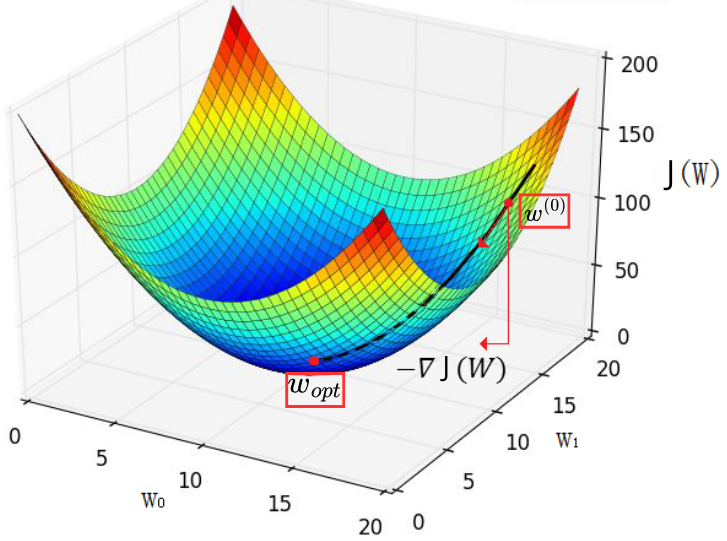
\includegraphics[width=0.8\linewidth]{grad.png}
    \caption{Illustration de la fonction quadratique $J(w)$}
\end{figure}

$$$$
\begin{align}
    y_c(n,\omega) &= \sum_{l=0}^{M-1} w_p x_c(n-l,w) \nonumber \\
    &= w * x_c(n,\omega) \nonumber \\
    &= \begin{pmatrix}
        w_0 & w_1 & \dots & w_{M-1} \\
    \end{pmatrix}
    \begin{pmatrix}
        x_c(n,\omega) \\
        x_c(n-1,w) \\
        \vdots \\
        x_c(n-M+1,w)
    \end{pmatrix} \nonumber \\
    &= \mathbf{w}^t \mathbf{x}(n,\omega) \nonumber
\end{align}

\begin{align}
    |e_c(n,\omega)|^2 &= \left( \mathbf{w^t} \mathbf{x}(n,\omega) - d_c(n,\omega) \right) \left( \mathbf{w}^t\mathbf{x}(n,\omega) - d_c(n,\omega) \right) ^\dag \nonumber \\
    &= \left( \mathbf{w}^t \mathbf{x}(n,\omega) - d_c(n,\omega) \right) \left( \mathbf{x}^\dag (n,\omega) + \mathbf{\overline{w}} - \overline{d_c(n,\omega)} \right)  \nonumber \\
    &= \mathbf{w}^t \mathbf{x}(n,\omega) \mathbf{x}^\dag (n,\omega) \overline{\mathbf{w}}  - \mathbf{w}^t \mathbf{x}(n,\omega) \overline{d_c(n,\omega)} - d_c(n,\omega) \mathbf{x}^\dag (n,\omega) \mathbf{\overline{w}} + |d_c(n,\omega)|^2 \nonumber
\end{align}
En faisant la moyenne sur $\omega \in \Omega$ :
\begin{align}
    J(w) &= E\left[ |e_c(n,\omega)|^2 \right] \nonumber \\
    &= \mathbf{w}^t E[\mathbf{x}(n,\omega) \mathbf{x}^\dag (n,\omega)] \overline{\mathbf{w}} - \mathbf{w}^t E[\mathbf{x}(n,\omega) \overline{d_c(n,\omega)}] - E[d_c(n,\omega) \mathbf{x}^\dag (n,\omega)] \mathbf{\overline{w}} + \sigma_d^2 \nonumber 
\end{align}
Par identification de :$$R_c = E[\mathbf{x}(n,\omega) \mathbf{x}^\dag (n,\omega)]$$
$$\mathbf{\gamma_{x,d}} = E[\mathbf{x}(n,\omega) \overline{d_c(n,\omega)}]$$
$$\mathbf{\gamma_{x,d}}^\dag = E[d_c(n,\omega) \mathbf{x}^\dag (n,\omega)]$$
Nous obtenons : $$J(w) = \mathbf{w}^t R_x \overline{\mathbf{w}} - \mathbf{w}^t \mathbf{\gamma_{x,d}}  - \mathbf{\gamma_{x,d}}^\dag \mathbf{\overline{w}} + \sigma_d^2$$

\textbf{Rappel :} $\dag$ signifie transposé $+$ conjugué d'un scalaire.  \\

Nous allons maintenant différencier le cas $\mathbf{w}$ et $\mathbf{w}+\delta \mathbf{w}$.\\
\begin{align}
    J(\mathbf{w}+\delta \mathbf{w}) &= (\mathbf{w}+\delta \mathbf{w})^t R_x \overline{(\mathbf{w}+\delta \mathbf{w})} - (\mathbf{w}+\delta \mathbf{w})^t \mathbf{\gamma_{x,d}} - \mathbf{\gamma_{x,d}}^\dag (\mathbf{w}+\delta \mathbf{w}) + \sigma_d^2 \nonumber \\
    &= J(w) + \delta \mathbf{w}^t R_x \overline{\mathbf{w}} - \delta \mathbf{w}^t \mathbf{\gamma_{x,d}} + \mathbf{w^t}R_c\delta\mathbf{w} - \mathbf{\gamma_{x,d}}^\dag \delta \mathbf{\overline{w}} + \delta \mathbf{w}^t R_x \delta \mathbf{\overline{w}} \nonumber
\end{align}

$$\Rightarrow \boxed{grad_\mathbf{\overline{w}} J(w) = 2(R_x \mathbf{\overline{w}} - \mathbf{\gamma_{x,d}})}$$
Gradient déterministe de l'erreur quadratique
\begin{itemize}
    \item $\mathbf{w}^{(0)}$ initial
    \item à l'itération $k$ : $\mathbf{\overline{w}^{(k)}} = \mathbf{\overline{w}^{(k-1)}} - \mu (R_x \mathbf{\overline{w}}^{k+1} - \mathbf{\gamma_{x,d}})$ 
    \item arrêt lorsque $k=k_{max}$ ou $\| \mathbf{w}^{k}-\mathbf{w}^{k-1} \| \leq \epsilon$
\end{itemize}
Il n'y a plus d'inversion de matrice \\ %%%%%%%%%%%%%%%%%%%%%%
\textbf{Question :} est de que $\mathbf{w}^{k} \underset{k \to +\infty}{\longrightarrow} \mathbf{w}_{\text{opt}}$ ?\\
Etude de convergence : $$\mathbf{\overline{w}^{(k)}} = \mathbf{\overline{w}^{(k-1)}} - \mu (R_x \mathbf{\overline{w}}^{k+1} - \mathbf{\gamma_{x,d}})$$
\begin{align}
    \Leftrightarrow \mathbf{\overline{w}^{(k)}} - \mathbf{\overline{w}_{opt}} &= \mathbf{\overline{w}^{(k-1)}} \mathbf{\overline{w}_{opt}} - \mu (R_x \mathbf{\overline{w}}^{k+1} - R_x \mathbf{\overline{w}_{opt}}) \nonumber \\
    &= \mathbf{\overline{w}^{(k-1)}} \mathbf{\overline{w}_{opt}} - \mu (R_x \mathbf{\overline{w}}^{k+1} - R_x \mathbf{\overline{w}_{opt}}) \nonumber \\
    &= (I_M - \mu R_x)(\mathbf{\overline{w}^{(k-1)}} - \mathbf{\overline{w}_{opt}}) \nonumber \\
    &= (I_M - \mu R_x)^{k}(\mathbf{\overline{w}^{(0)}} - \mathbf{\overline{w}_{opt}}) \nonumber \\
\end{align}
$$R_x = U \Lambda U^\dag$$ 
U matrice unitaire car $R_x^\dag = R_x$
et $\Lambda = diag(\lambda_1, \lambda_2, \dots ,\lambda_M)$
$u \neq 0$ $$\mathbf{u^\dag} R_x \mathbf{u}=\mathbf{u^\dag} E[\mathbf{x}(n,\omega) \mathbf{x}^\dag (n,\omega)]\mathbf{u} $$
$$= E\left[ |\mathbf{u}^\dag \mathbf{x}(n,\omega) |^2 \right]$$
$$\text{réel }>0 \text{ sauf } \mathbf{x}(n,\omega)=0 $$
$$\Rightarrow \lambda_1 > 0 \Rightarrow R_x \text{ inversible}$$
$$I_M - \mu R_x = UU^+ - \mu U\Lambda U^\dag = U\cdot diag(1- \mu \lambda_1, \dots, 1- \mu \lambda_M)\cdot U^\dag$$
$$(I_M - \mu R_x)^2 = UDU^+ \cdot UDU^\dag = UD^2U^\dag \text{ car } U^\dag U = I_M$$
$$(I_M - \mu R_x)^k = UD^kU^\dag$$
Donc $\mathbf{w}^{k} \underset{k \to +\infty}{\longrightarrow} \mathbf{w}_{\text{opt}}$ ssi $(1 - \mu \lambda_i)^k \underset{k \to +\infty}{\longrightarrow} 0 $
$$\Leftrightarrow |1- \mu \lambda_i|< 1$$
ATTENTION : Si un des $|1- \mu \lambda_i|> 1$ alors il y aura divergence.\\
Convergence $\Leftrightarrow -1 <1 - \mu \lambda_i < 1 \Leftrightarrow 0< \mu < \frac{2}{\lambda_1} \Leftrightarrow \boxed{0 < \mu < \frac{2}{\lambda_{max}(R_x)}}$  \\
Pas d'inpact de $\mathbf{w}^{(0)}$.\\
Remarque : S'il existe $k_0$ tel que $R_x \mathbf{\overline{w}}(k_0) - \mathbf{\gamma_{d,x}}=0$ l'algorithme s'arrête.\\
La vitesse de convergence est proportionnelle à $max|1-\mu \lambda_i|= 1-\mu \lambda_{min}(R_x)$. La fonction de conditionnement de $R_x$ est $\frac{\lambda_{min}(R_x)}{\lambda_{max}(R_x)}$.\\
Si $\lambda_{min} \simeq \lambda_{max} $ favorable, sinon $\lambda_{min} << \lambda_{max} $ alors $R_x$ est mal conditionné.\\
En pratique 
\begin{align}
    trace(R_x) &= \gamma_x(0) M = M\sigma_x^2 \nonumber \\
    &= \sum_i \lambda_i \leq M \lambda_{max}(R_x)
\end{align}
$$\frac{2}{M\sigma_x^2} \leq \frac{2}{\sigma_{max}(R_x)} < \frac{2}{M\sigma_x^2} $$
$$\hat{\sigma_x^2} = \frac{1}{M} \sum_{m=0}^{M-1}|x_c(n-m,w)|^2 = \| \mathbf{x}(n,\omega) \|^2$$
Il faut $R_x := \hat{\gamma_x}(0), \dots ,\hat{\gamma_x}(M-1) $ et $ \mathbf{\gamma_{x,d}} := \hat{\gamma_{x,d}}(0), \dots ,\hat{\gamma_{x,d}}(M-1) \Rightarrow$ coût estimation.

On voudrait : 
\begin{enumerate}
    \item éviter le coût de l'estimation 
    \item ne pas avoir besoin de la stationnarité ie. s'adapter aux variations des statiques des signaux.
\end{enumerate}
\subsection{Gradient stochastique de l'erreur quadratique : LMS}
Idée : $ J(\mathbf{w}) \rightarrow \Tilde{J}(\mathbf{w}) = |e_c(n,\omega)|^2$ on a enlevé E avec un gradient stochastique (fonction de la réalisation $w$) pour garder de la mémoire des instants précédents. 
\begin{itemize}
    \item $\mathbf{w}^{(0)}$ initialisation
    \item à l'instant $n$ : $\mathbf{\overline{w}^{(n)}} = \mathbf{\overline{w}^{(n-1)}} - \mu grad_{\mathbf{w}}\Tilde{J}(\mathbf{w)} \Big|_{\mathbf{w} = \mathbf{w}^{n-1}}$ 
\end{itemize}
Aune réalisation donnée : $$\Tilde{J}(\mathbf{w}) = \mathbf{w^t} \mathbf{x(n,\omega)} \mathbf{x^\dag (n,\omega)} \mathbf{\overline{w}}  - \mathbf{w^t} \mathbf{x(n,\omega)} \overline{d_c(n,\omega)} - d_c(n,\omega) \mathbf{x^\dag (n,\omega)} \mathbf{\overline{w}} + |d_c(n,\omega)|^2 $$
\begin{align}
    grad_\mathbf{\overline{w}} \Tilde{J(w)} 
    &= 2(\mathbf{x}(n,\omega)\mathbf{x}^\dag(n,\omega) - \mathbf{x}(n,\omega)\overline{d_c(n,\omega)}) \nonumber \\
    &=2(R_x \mathbf{\overline{w}} - \mathbf{\gamma_{x,d}}) \text{ par analogie} \nonumber 
\end{align}
Cette fois nous ne prenons pas l'espérence donc nous pouvons factoriser l'expression.
\begin{align}
    grad_\mathbf{\overline{w}} \Tilde{J(w)} 
    &= 2 \mathbf{x}(n,\omega)(\mathbf{x}^\dag(n,\omega) - \overline{d_c(n,\omega)}) \nonumber \\
    &= \overline{\mathbf{w}^t\mathbf{x}(n,\omega) - d_c(n,\omega)} \nonumber
\end{align}
Algorithme Least Mean Square (LMS) : \\
à l'instant n : 
$$e_c^{(n)} = \mathbf{w}^{(n-1)t}\mathbf{x}(n,\omega) - d_c(n,\omega)$$
$$\overline{\mathbf{w}}^{(n)} = \overline{\mathbf{w}}^{(n-1)} - \mu \overline{e_c^{(n)}(n,\omega)}\mathbf{x}(n,\omega)$$
Il y a une mise à jour dans la direction du vecteur de régression. On met un critère d'arrêt si c'est pour de l'apprentissage (pas si on continue à s'adapter).\\
C'est un algorithme de traitement du signal et d'apprentissage largement utilisé du fait de sa faible complexité de son aspect adaptatif.\\
\textbf{Convergence :} cas de signaux stationnaires $\mathbf{w}_{opt}$ connu.\\
En moyenne sur les réalisations $w$ : $$E[\overline{\mathbf{w}^{(n)}}] = E[\overline{\mathbf{w}^{(n-1)}}] - \mu E[(\overline{\mathbf{w}^{(n-1)t}\mathbf{x}(n,\omega) - d_c(n,\omega)})x_c(n,\omega)]  $$
Hypothèse fausse : $\mathbf{w}^{(n-1)}$ décorrélé de $\mathbf{x}(n,\omega)$. On retrouve $grad_\mathbf{\overline{w}} J(w)$
\\
Equation du gradient déterministe en $E[\mathbf{\overline{w}^{(n)}}]$ :
$$E[\overline{\mathbf{w}^{(n)}}] = E[\overline{\mathbf{w}^{(n-1)}}] - \mu \left(R_x E[\overline{\mathbf{w}^{-(n-1)}}]- \mathbf{\gamma_{x,d}}\right) $$
Et on a convergence si le pas respect la condition suivante : 
$$0<\mu<\frac{2}{\lambda_{max}(R_x)}$$
Théorie de l'ODE, cette théorie montre que cette hypotèse même fausse nous donne bien le comprtement de l'algorithme si le pas est faible. (Pour aller plus loin scénario de Macchi - LMS).\\

\textbf{Exercice 1:}\\
$\Tilde{e}_c(n,\omega)$ : erreur a posteriori\\
$\Tilde{e}_c(n,\omega) = \mathbf{w}^{(n)t}\mathbf{x}(n,\omega) - d_c(n,\omega)$\\
Calculer $\Tilde{e}_c(n,\omega)$. Comment adapter le pas $\mu$ pour annuler cette erreur ?\\
\begin{align}
    \Tilde{e}(n,\omega) &= \mathbf{w}^{(n)t}\mathbf{x}(n,\omega) - d_c(n,\omega) \nonumber \\
    &= \left( \mathbf{w}^{(n-1)} - \mu e_c^{(n)}(n,\omega) \overline{\mathbf{x}}(n,\omega) \right)^t \mathbf{x}(n,\omega) - d_c(n,\omega) \nonumber \\
    &= \mathbf{w}^{(n-1)t} \mathbf{x}(n,\omega) - \mu  e_c^{(n)}(n,\omega) \| x(n,w) \|^2 -  d_c(n,\omega) \nonumber \\
    &= e_c^{(n)}(n,\omega) \left( 1- \mu \| x(n,w) \|^2 \right)
\end{align}
Ainsi $\Tilde{e}(n,\omega)=0 $ ssi $\mu = \frac{1}{\| x(n,w) \|^2}$. \\
On appelle cela \textit{Normalized LMS (NLMS)} \\
$$\overline{\mathbf{w}}^{(n)} = \overline{\mathbf{w}}^{(n-1)} - \frac{\mu}{\| x(n,\omega) \|^2} \overline{e_c}^{(n)}(n,\omega) \mathbf{x}(n,\omega) $$
On normalise a chaque fois l'entré $x$ par sa norme et on normalise aussi la référence :
$$\mu \left( \overline{\mathbf{w}}^{(n-1)} \frac{\mathbf{x}}{\|x\|} - \frac{d_c}{\|x\|}\right) \frac{\mathbf{x}}{\|x\|}$$
Cela revient à normaliser l'\textbf{observateur} $\frac{\mathbf{x}(n,\omega)}{\|\mathbf{x}(n,\omega)\|}$ et la \textbf{référence} $\frac{d_c(n,\omega)}{\|\mathbf{x}(n,\omega)\|}$.\\
Interessant pour tous les signaux dont l'amplitude varie beaucoup.\\

Concernant les performances, il faut trouver un compromis sur le pas $\mu$ : 
\begin{enumerate}
    \item $\mu$ très faible : convergence lente, moins d'adaptation aux variations des statiques des signaux.
    \item $\mu$ assez grand mais pas trop, pour qu'il y ait toujours convergence : bruit trop important
    \item $\mu$ trop grand : divergence
\end{enumerate}

\subsection{Recursive Least Square (RLS)}
On veut un interméddiare entre : $J(\mathbf{w}) = E \left[ |e|^2 \right]$ et $\Tilde{J}(\mathbf{w}) = |e|^2$\\
Moyenne temporelle : $$\Tilde{\Tilde{J}}(\mathbf{w}) = \sum_{i=0}^{\infty} \beta(i) |e_c(n-i,\omega)|^2$$
$\beta(i)$ est la pondération, il ajoute plus de poids aux instants juste avant n.
On peut choisir pour $\beta (i)$ une fenêtre glissante~Figure \ref{fig:porte} (ie un fonction porte de vallant 1 si $i \ in [0,L-1]$ ou bien nous pouvons introduire un facteur d'oublie $\lambda \in [0,1]$ tel que $\beta(i) = \lambda^i$ Figure \ref{fig:oublie}. 
\begin{figure}[H]
    \centering
    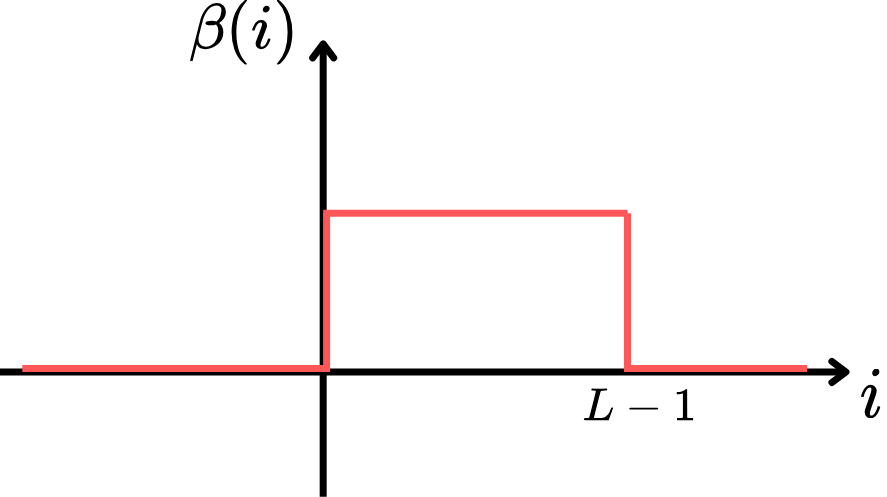
\includegraphics[width=0.5\linewidth]{porte.png}
    \caption{Fenêtre glissante}
    \label{fig:porte}
\end{figure}

\begin{figure}[H]
    \centering
    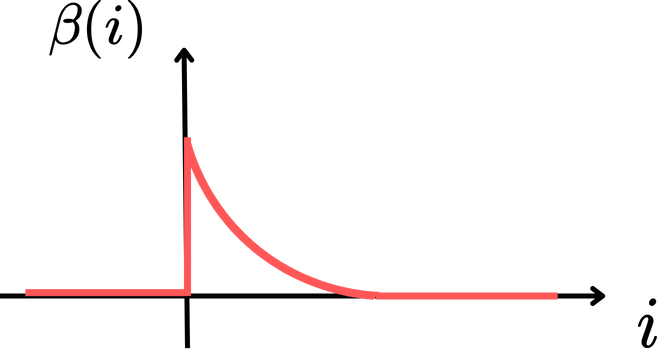
\includegraphics[width=0.5\linewidth]{oublie.png}
    \caption{Facteur d'oublie}
    \label{fig:oublie}
\end{figure}


En pratique, $\lambda$ est choisi tel qu'il est très proche de 1 (ie 0.99).\\
Si $\lambda \rightarrow 1$ : gradient déterministe.\\
Si $\lambda \rightarrow 0$ : LMS.\\

$$\mathbf{w}^{(n)} = arg\min_{\mathbf{w}} \Tilde{\Tilde{J}}(\mathbf{w})$$
vérifie $$R_x(n) \overline{\mathbf{w}}^{(n)} = \mathbf{\gamma}_{x,d}(n)$$
avec 
\begin{align}
    R_x(n) &= \sum_{l=-\infty}^n \lambda^{n-l} \mathbf{x}(l,\omega) \mathbf{x}^+(l,\omega)  \nonumber \\
    &= \lambda \sum_{l=-\infty}^{n-1} \lambda^{n-l-1} \mathbf{x}(l,\omega) \mathbf{x}^+(l,\omega) + \mathring{\lambda} \mathbf{x}(n,\omega) \mathbf{x}^+(n,\omega) \nonumber \\
    &= \lambda R_x(n-1) + \mathbf{x}(n,\omega) \mathbf{x}^+(n,\omega) \nonumber
\end{align}

\begin{align}
    \mathbf{\gamma}_{x,d}^{(n)} =& \sum_{l=-\infty}^{n} \lambda^{n-l} \mathbf{x}(l,\omega) \overline{d_c}(l,\omega) \nonumber \\
    &= \lambda \gamma_{x,d}(n-1) + \mathbf{x}(n,\omega) \overline{d_c}(n,\omega) \nonumber
\end{align}

Pour avoir une récursion sur $\mathbf{w}$, il faut une récursion sur $(R_x(n))^{-1} = S(n)$.\\

\textbf{Lemme d'inversion matricielle :} Si $A= B + \mathbf{u} \mathbf{u}^\dag$ et B est inversible alors $$A^{-1} = B^{-1} - \frac{B^{-1} \mathbf{u} \mathbf{u}^\dag B^{-1}}{1+  \mathbf{u}^\dag B^{-1}\mathbf{u}}$$
$B = \lambda R_x(n-1)$ et $B^{-1} = \frac{1}{\lambda}S(n-1)$ et $\mathbf{u} = \mathbf{x}(n,\omega)$
\begin{align}
    \Leftrightarrow S(n) &= \frac{1}{\lambda} S(n-1) \nonumber \\
    &= \frac{1}{\lambda} \frac{S(n-1) \mathbf{x}(n,\omega) \mathbf{x}^+(n,\omega) S(n-1)}{1+1/ \lambda   \mathbf{x}^+(n,\omega) S(n-1 \mathbf{x}(n,\omega)} \nonumber 
\end{align}

\begin{equation}
    \mathbf{k}(n,\omega) = \frac{1}{\lambda} \frac{S(n-1) \mathbf{x}(n,w)}{1 + \frac{1}{\lambda} \mathbf{x}^\dag(n,\omega) S(n-1) \mathbf{x}(n,\omega)} \nonumber
\end{equation}
\begin{equation}
    s(n) = \frac{1}{\lambda} S(n-1) - \frac{1}{\lambda} \mathbf{k}(n,\omega) \mathbf{x}^\dag(n,\omega) S(n-1) \nonumber
\end{equation}
\begin{equation}
    (13) \Leftrightarrow \left( 1 + \frac{1}{\lambda} \mathbf{x}^\dag(n,\omega) S(n-1) \mathbf{x}(n,\omega) \right) \mathbf{k}(n,\omega)=\frac{1}{\lambda}S(n-1)\mathbf{x}(n,\omega) \nonumber
\end{equation}
\begin{align}
    \mathbf{k}(n,\omega) &= \frac{1}{\lambda}S(n-1) \mathbf{x}(n,\omega) - \frac{1}{\lambda} \mathbf{x}^+(n,\omega) S(n-1)\mathbf{x}(n,\omega) \mathbf{k}(n\omega) \nonumber \\
    &= \frac{1}{\lambda} S(n-1) - \frac{1}{\lambda} \mathbf{k}(n,\omega) \mathbf{x}^+(n,\omega) S(n-1) \mathbf{x}(n\omega) \nonumber \\
    &= S(n,\omega) \mathbf{x}(n,\omega) \nonumber
\end{align}
\begin{align}
    \overline{\mathbf{w}}^{(n)} &= S(n) \mathbf{\gamma}_{x,d}(n) \nonumber \\
    &= \left( \frac{1}{\lambda} S(n-1) - \frac{1}{\lambda} \mathbf{k}(n,\omega) \mathbf{x}^+(n,\omega) S(n-1) \right) \left( \lambda \mathbf{\gamma}_{x,d}(n-1) + \mathbf{x}(n,\omega)\overline{d_c}(n,\omega) \right) \nonumber \\
    &= S(n-1) \mathbf{\gamma}_{x,d}(n-1) - \mathbf{k}(n,\omega) \mathbf{x}^+(n,\omega) S(n-1) \mathbf{\gamma}_{x,d}(n-1) + S(n) \mathbf{x}(n,\omega)\overline{d_c}(n,\omega) \nonumber  \\
    &= \overline{\mathbf{w}}^{(n-1)} - \mathbf{k}(n,\omega) \mathbf{x}^+(n,\omega) \overline{\mathbf{w}}^{(n-1)}+ \mathbf{k}(n,\omega) \overline{d_c}(n,\omega) \nonumber \\
    &= \overline{\mathbf{w}}^{(n-1)} - \mathbf{k}(n,\omega) \left( \mathbf{x}^+(n,\omega) \overline{\mathbf{w}}^{(n-1)}+ \overline{d_c}(n,\omega) \right) \nonumber \\
    &= \overline{\mathbf{w}}^{(n-1)} - \overline{e_c}^{(n)}(n,\omega) \mathbf{k}(n,\omega) \nonumber 
\end{align}
\subsubsection{Algo RLS :}
\begin{itemize}
    \item $\mathbf{w^{(0)}}$
    \item à chaque instant n : $\mathbf{k}(n,\omega) = \frac{S(n-1) \mathbf{x}(n,w)}{\lambda +  \mathbf{x}^\dag(n,\omega) S(n-1) \mathbf{x}(n,\omega)}$ Le numérateur est l'inversion Hessienet le dénominatuer n'est pas adaptatif.
    \item $e_c^{(n)}(n,\omega) = w^{(n-1)b}\mathbf{x}(n,\omega) - d_c(n,\omega)$
\end{itemize}
$$\overline{\mathbf{w}}^{(n)} = \overline{\mathbf{w}}^{(n-1)} - \overline{e_c}^{(n)}(n,\omega) \mathbf{k}(n,\omega)$$
On pose $\mathbf{u} = S(n-1)\mathbf{x}(n,\omega)$
$$S(n) = \frac{1}{\lambda}S(n-1) - \frac{1}{\lambda} \mathbf{k}(n,\omega) \mathbf{x}^+(n,\omega) S(n-1) $$
On reconnait : $ \mathbf{u}^\dag = \mathbf{x}^\dag (n,\omega) S(n-1) $\\
\textbf{RLS} : 
\begin{itemize}
    \item stochastique
    \item adaptation
    \item plus comlpexe que LMS, convergence beaucoup plus rapide que LM
    \item $\lambda \rightarrow 1$ moyennage mieux si signaux stationnaire 
    \item $\lambda \rightarrow 0.99$
\end{itemize}

\textbf{Exercice : } Prédiction linéaire à 3 pas\\
Ecrire l'algorithme LMS. On se place à l'instant n et on veut prédire $x(n+3)$. C'est à dire que l'on veut apprendre et adapter un filtre de prédiction d'ordre M.
\begin{itemize}
    \item Expliciter $d(n,\omega)$ puis $\gamma_{x,d}(p)$
    \item Que doit vérifier $\mathbf{w}_{opt}$ avec M=2.
    \item Cas particulier $\gamma_x(p) = \frac{a^2}{2}cos(2 \pi \nu p)$ (sinusoïde à phase aléatoire)
\end{itemize}


\textbf{Exercice :} Pour faire la prédiction à 3 pas, obtient-on le même résulata en faisant 3 fois la prédiction à 1 pas ? \\
On fera l'hypothèse de stationnarité. 
\subsection{Filtre de Kalman}
Le filtre de Kalman doit son nom à Rudolf Kalman bien que Andreï Nikolaïevitch Kolmogorov, un mathématicien russe et soviétique ait développé un algorithme similaire avant lui portant sur les moèles d'états étudiés en automaatique. \\
Idée de Kalman porte sur la prédiction linéaire sur un modèle d'état.\\

\textbf{Modèle d'état (simple)} :\\
équation d'observation :
$$x(n,\omega) = \mathbf{c}^t \mathbf{z}(n,\omega) + b_1(n,\omega)$$
équation d'état : 
$$\mathbf{z}(n+1,\omega) = A \mathbf{z}(n,\omega) + b_2(n,\omega) \text{ (bruit du modèle)}$$

\textbf{Exemple :} trajectoires (robot, automobile) pistage de vision de système dynomique\\
Accélération constante : $\Ddot{z}_{n+1} = \Ddot{z}_n$\\
Vitesse : $\Dot{z}_{n+1} = \Dot{z}_n + \alpha \Ddot{z}_n$ \\
Position : $z_{n+1} = z_n + \alpha \Dot{z}_n + \frac{\alpha^2}{2} \Ddot{z}_n$ \\
Vecteur d'état : $\mathbf{z}_n = \begin{pmatrix}
    z_n \\
    \Dot{z}_n \\
    \Ddot{z}_n
\end{pmatrix}$
$$x(n,\omega) = z_n + b_n(n,\omega)$$
On introduit un bruit d'observation $b_n$ à la vrai position $z_n$\\
\textbf{Question :} Comment améliorer la prédiction linéaire de $x$ en utilisant le modèle d'état ? \\
Etant donné $x(n), x(n+1), \dots, x(n-M+1)$, comment prédire $\hat{x}(n+1) = y_{opt}(n)$
\begin{align}
    y_{opt} &= \hat{x}(n+1) = w_{opt} * x(n) \nonumber \\
    &= x(n+1)\|x(n) \text{ (projection orthogonal)} \nonumber
\end{align}
$x_n$ est une combinaison linéaire de $x_n, x_{n+1}, \dots x_{n-M+1}$\\
Or $x(n++1) = \hat{x}(n+1) + e_n(n-1)$
$$\Leftrightarrow x_n = x_n \oplus e_{opt}(n+1)$$
On va utiliser le modèle d'état : 
\begin{align}
    \hat{x}(n+1) &= x(n+1)\| x_n \nonumber \\
    &= \left( \mathbf{c}^t \mathbf{z}(n+1) + b_1(n+1) \right)\| x_n \nonumber \\
    &= \mathbf{c}^t \mathbf{z}(n+1) \| x_n + b_1(n+1) \| x_n \text{ (par linéarité)} \nonumber \\
    &= \mathbf{c}^t \mathbf{z}(n+1) \| x_n \nonumber
\end{align}
On note $\hat{\mathbf{z}}(n+1) = \mathbf{z}(n+1) \| x_n$ et $\mathbf{\epsilon}(n+1) = \hat{z}(n+1) - \mathbf{z}(n+1)$, il s'agit de l'erreur de prédiction sur l'état
$$e(n+1) = \hat{x}(n+1) - x(n+1) = \mathbf{c}^t \hat{\mathbf{z}}(n+1) - (\mathbf{c}^t \hat{\mathbf{z}}(n+1) + b_1(n+1))$$
\begin{align}
    \hat{\mathbf{z}}(n+1) &= \mathbf{z}(n+1) \|x_n \nonumber \\
    &= (A\mathbf{z}(n) + b_2(n))\| x_n \nonumber \\
    &= A \mathbf{z}(n) \| x_n + b_2(n) \| x_n \nonumber
\end{align}
On note :
\begin{align}
    \hat{\mathbf{z}}(n) &= \mathbf{z}_n \| x_n \nonumber \\
    &= \mathbf{z}_n \| (x_n \oplus \{e_{opt}(n) \}) \nonumber \\
    &= \mathbf{z}_n \| x_n + \mathbf{z}_n  \| \{e_{opt}(n) \} \nonumber \\
    &= \mathbf{z}_n + E \left[ \mathbf{z}_c(n) \overline{e_{opt,c}(n)} \right] \left( E \left[ \mathbf{z}_c(n) \overline{e_{opt,c}(n)} \right] \right)^\dag e_{opt}(n) \nonumber
\end{align}
$E \left[ \mathbf{z}_c(n) \overline{e_{opt,c}(n)} \right] \left( E \left[ \mathbf{z}_c(n) \overline{e_{opt,c}(n)} \right] \right)^\dag$ : ce terme est appelé le gain de Kalman.\\
Il ne reste plus qu'à calculer le gain de Kalman.

\begin{align}
    E \left[ e_{opt,c}(n) \overline{e_{opt,c}(n)} \right] &= E\left[ (\mathbf{c}^t \mathbf{\epsilon}_c(n) - b_{1,c}(n)) \overline{(\mathbf{c}^t \mathbf{\epsilon}_c(n) - b_{1,c}(n))} \right] \nonumber \\
    &= \mathbf{c}^t E[\mathbf{\epsilon}_c(n) \mathbf{\epsilon}_c^\dag(n)]\mathbf{c} + \sigma_{bn}^2 \nonumber \\
    E \left[ z_c(n) \overline{e_{opt}(n)} \right] &= E\left[\mathbf{z}_c (\mathbf{c}^t \mathbf{\epsilon}_c(n) - b_{1,c}(n)) \right] \nonumber \\
    &= E[ \mathbf{z}_c(n) \mathbf{\epsilon}_c^\dag (n)] \mathbf{c} - E[ \mathbf{z}_c(n) b_{1,c}(n)] \text{ 2e terme =0}\nonumber \\
    &= E[ (\hat{\mathbf{z}}_c(n) - \mathbf{\epsilon}_c (n)) \mathbf{\epsilon}_c^\dag (n)] \mathbf{c} \nonumber \\
    &= E[ \hat{\mathbf{z}}_c(n) \mathbf{\epsilon}_c^\dag (n)] - E[ \mathbf{\epsilon}_c (n)) \mathbf{\epsilon}_c^\dag (n)] \mathbf{c} \text{ 1er terme =0 car $\perp$ prédiction} \nonumber \\
    &= -P_n \mathbf{c} \nonumber
\end{align}
\textbf{Remarque : } $E[\mathbf{\epsilon}_c(n) \mathbf{\epsilon}_c^\dag(n)]$ peut être noté $P_n$
$$\Rightarrow \mathbf{G_n} = - P_n \mathbf{c}(\mathbf{c}^t P_n \mathbf{c} + \sigma_{bn}^2)\dag$$
Mise à jour de $P_n$, on a : 
\begin{align}
    \epsilon(n) &= \hat{z}(n+1) - z(n+1) \nonumber \\
    &= A (\hat{z} + G(n)e_{opt}(n)) - (A z(n) + b_2(n)) \nonumber \\
    &= A(\hat{z}(n) - z(n)) + A  G(n) e_{opt} - b_2(n) \text{ par identification de $\hat{z}(n) - z(n)= \epsilon(n)$ } \nonumber \\
    &= A(\epsilon(n) + G(n) e_{opt}(n)) - b_2(n) \text{décorrelés} \nonumber \\
    P_{n+1} = E[\mathbf{\epsilon}_c(n) \mathbf{\epsilon}_c^\dag(n)] \nonumber \\
    &= A Cov(\epsilon(n) + G(n) e_{opt}(n))A^\dag -+ Cov(b_2(n)) \nonumber
\end{align}

Pour un filtre de Kalman $cov(b_2)$ est connue\\
Initialisation : $\hat{z}(0)$, $P_0$\\
A l'instant n : $$e(n) = c^t \hat{z}(n) - x(n)$$
$$G(n)=-P_n c(c^t P_n c + \sigma^2)^{-1} $$
$$c(n+1) = A(\hat{z}(n) + G(n) e(n))$$
$$P_n^{(n)} = (I-G(n)c)P_n$$
$$P_{n+1} = AP_n^{(n)} A^\dag + Cov(b_2)$$

\newpage
\subsection{Algorithme EM (Expectation-Maximization)}
L'algorithme espérance-maximisation est un algorithme itératif qui permet de trouver les paramètres du maximum de vraisemblance d'un modèle probabiliste lorsque ce dernier dépend de variables latentes non observables.\\
On utilise souvent l'algorithme EM pour la classification de données (clustering, ou partitionnement de données), l'apprentissage automatique, ou la vision artificielle. (imagerie médicale dans le cadre de la reconstruction tomographique)\\

L'algorithme d'espérance-maximisation consiste à itérer les deux étapes suivantes : \\
étape E : une étape d'évaluation de l'espérance, où l'on calcule l'espérance de la vraisemblance en tenant compte des dernières variables observées,\\
étape M : une étape de maximisation, où l'on estime le maximum de vraisemblance des paramètres en maximisant la vraisemblance trouvée à l'étape E.\\
On utilise à chaque fois les paramètres trouvés en l'étape M comme point de départ d'une nouvelle étape E d'évaluation de l'espérance.\\

\textbf{Etape E :}\\
Estimation des données inconnues, sachant les données observées et la valeur des paramètres determinés à l’itération précédente.\\
Calcul des probabilités conditionnelles $t_{ik}^{(c)}$ :\\

L'espérance conditionnelle est donnée par :
\[
\mathbb{E}[z_{ik} \mid x_i, \theta^{(c)}] = t_{ik}^{(c)} = \mathbb{P}(z_{ik} = 1 \mid x_i, \theta^{(c)}).
\]

En appliquant la règle de Bayes, on obtient :
\[
\mathbb{P}(z_{ik} = 1 \mid x_i, \theta^{(c)}) = \frac{\mathbb{P}(z_{ik} = 1, x_i \mid \theta^{(c)})}{\mathbb{P}(x_i \mid \theta^{(c)})}.
\]

Le numérateur se ré-écrit sous la forme :
\[
\mathbb{P}(z_{ik} = 1, x_i \mid \theta^{(c)}) = \pi_k^{(c)} p(x_i \mid \theta_k^{(c)}),
\]

Et le dénominateur est la probabilité marginale :
\[
\mathbb{P}(x_i \mid \theta^{(c)}) = \sum_{j=1}^K \pi_j^{(c)} p(x_i \mid \theta_j^{(c)}).
\]

Donc :
\[
t_{ik}^{(c)} = \frac{\pi_k^{(c)} p(x_i \mid \theta_k^{(c)})}{\sum_{j=1}^K \pi_j^{(c)} p(x_i \mid \theta_j^{(c)})}.
\]

Pour \( K = 2 \) :
\[
t_{ik}^{(c)} = \frac{\pi_k^{(c)} p(x_i \mid \theta_k^{(c)})}{\pi_1^{(c)} p(x_i \mid \theta_1^{(c)}) + \pi_2^{(c)} p(x_i \mid \theta_2^{(c)})}.
\]
De plus, la marginalisation estimée de la fonction de log-vraisemblance sachant la valeur courante des paramètres du mélange $\theta (c)$  est donnée par :
\[
Q(\theta, \theta^{(c)}) = E(\log p(x,z |\theta) |x, \theta^{(c)})
\]
Et :
\[
\ln(p(x,z|\theta) = E_z(\ln p(x|\theta,z)) = \sum_{i=1}^{N} \sum_{k=1}^{2} z_{ik} ln(\pi_k p(x|\theta, z_{ik}))
\]
En combinant, nous obtenons bien : 
\[
Q(\theta, \theta^{(c)}) = \sum_{i=1}^{N} \sum_{k=1}^{2} t_{ik}^{(c)} ln(\pi_k^{(c)} p(x_i|\bf{\theta}, z_{ik}))
\]
\textbf{Etape M :}\\
Maximisation de la vraisemblance, rendue désormais possible en utilisant l’estimation des données inconnues effectuée à l’étape précédente, et la mise à jour de la valeur du ou des paramètres pour la prochaine itération.\\
Ici nous nous intéressons à $Q(\pi_k)$.
\[
\begin{aligned}
Q(\theta, \theta^{(c)}) &= \sum_{i=1}^{N} \sum_{k=1}^{2} t_{ik}^{(c)} \ln(\pi_k^{(c)} p(x_i|\boldsymbol{\theta}, z_{ik})) \\
&= \sum_{i=1}^{N} \sum_{k=1}^{2} t_{ik}^{(c)} \ln(\pi_k^{(c)}) + \sum_{i=1}^{N} \sum_{k=1}^{2} t_{ik}^{(c)} \ln(p(x_i|\boldsymbol{\theta}, z_{ik})).
\end{aligned}
\]

Nous devons prendre en compte la contrainte : $\pi_1 + \pi_2 = 1$. Pour intégrer cette contrainte dans notre fonction, nous pouvons introduire un multiplicateur de Lagrange : $\lambda$

\[
L(\pi_k, \lambda) = \sum_{i=1}^{N} \sum_{k=1}^{2} t_{ik}^{(c)} ln(\pi_k^{(c)}) + \lambda (1- \sum \pi_k)
\]

En dérivant :
\[
\frac{\partial L}{\partial \pi_k} = \frac{1}{\pi_k} \sum_{i=1}^{N} t_{ik}^{(c)} - \lambda
\]

\[
\frac{\partial L}{\partial \pi_k} = 0 \Leftrightarrow \pi_k \lambda = \sum_{i=1}^{N} t_{ik}
\]

\[
 (\lambda \neq 0) \Rightarrow \pi_k  = \frac{\sum_{i=1}^{N} t_{ik}}{\lambda}
\]
Or, $\pi_1 + \pi_2 = 1$ : 
\[
  \frac{\sum_{i=1}^{N} t_{i1}}{\lambda} +\frac{\sum_{i=1}^{N} t_{i2}}{\lambda} = 1
\]
Donc $$\lambda = \sum_{i=1}^{N} t_{i1}+ t_{i2} = N$$ 
Car, $\forall i \sum_k t_{ik}=1$ puisque $t_{ik}$ est une distribution de probabilité sur les composantes de chaque $x_i$. d'après l'expression de $t_{ik}$.\\
Et nous avons : 
\[
m_1^{(c+1)} = \frac{\sum_{i=1}^{n} t_{ik} x_i}{\sum_{i=1}^{n} t_{ik}}
\]

\[
\sigma_1^{2(c+1)} = \frac{\sum_{i=1}^{n} t_{ik} (x_i-m_k)(x_i-m_k)}{\sum_{i=1}^{n} t_{ik}}
\]

\end{document}


